\paragraph{Experimente:}
\begin{itemize}
  \item gleichnamige Pole stoßen sich ab
  \item ungleichnamige Pole ziehen sich an\\
  \item Kraftwirkung $\propto\frac{1}{r^2}$ (1750; Coulomb)
  \item ähnliche Abstandsabhängigkeit für elektrische und für magnetische Kräfte
  \item zunächst kein Zusammenhang zwischen beiden Kräften erkennbar
  \item Experiment: Magnetische Pole treten nur paarweise auf. \\ ($\implies$ keine "magnetische Ladung")
\end{itemize}

\paragraph{Feldlinien sichtbarmachen durch Eisenfeilspitzen:}\leavevmode \\

\boxed{Magnetische Feldlinien sind stets geschlossen; es gibt keine isolierbaren Quellen oder Senken des magnetischen Felds.}

\paragraph{Erinnerung: Satz von Gauß:}\leavevmode \\
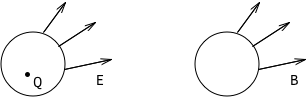
\includegraphics{skizzen/16/16_0B01}

$\vec{E}:$ elektrische Feldstärke:\\
Gesamtfluss: $\phi_{el}=\oint_A \vec{E}\cdot d\vec{A}=\frac{Q}{\epsilon_0}$\\

\subparagraph{Magnetische Felder:}\leavevmode \\

Gesamtfluss: $\boxed{ \phi_{mag}=\oint_A \underbrace{\vec{B}\cdot d\vec{A}}_{\text{magnetischer Fluss}}=0 \\ \vec{B}: \text{magnetische Flussdichte}}$
  
  \subsection{ Kräfte auf bewegte Ladungen }  
    \subsubsection{ Lorentzkraft $\vec{F}_L$ }
    $\vec{F}_L = q\cdot\vec{v}\times\vec{B}\\ (\vec{F}_L \perp \vec{v}; \vec{F}\perp \vec{B} ) $\\
    
    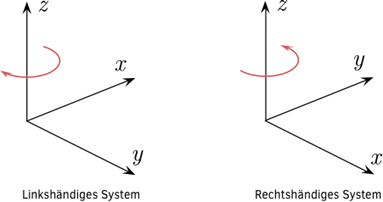
\includegraphics{skizzen/16/16_1B01}\\
    
    UVW-Regel: Ursache $\rightarrow$ Vermittler $\rightarrow$ Wirkung\\
    Vorsicht!: Elektrische Ladung ist negativ!\\
    
    $[\vert\vec{B}\vert]=\frac{N}{As\cdot\frac{m}{s}}=\frac{Vs}{m^2}=1T (Tesla)$
    
    Kreisbahn: $\vec{F}_L\perp \vec{v}$
    
    $\implies \vec{F}_L$ beeinfluss die Richtung von $\vec{v}$, aber nicht den Betrag!\\
    $\implies \vec{F}_L$ leistet keine Arbeit
    
      \paragraph{Konventionen:}\leavevmode \\
      
      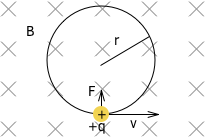
\includegraphics{skizzen/16/16_1B02}\\
      
      $\otimes \vec{B}$ zeigt in die Papierebene hinein\\
      
      $\odot \vec{B}$ zeigt aus der Papierebene heraus\\
      
      
  \subsubsection{Bewegungsgleichung:}\leavevmode \\
  
  $m\ddot{\vec{r}} = \dot{\vec{r}}=\vec{F}_L=q\cdot\vec{v}\times\vec{B} $\\
  
  $\frac{d\vec{v}}{dt}=\dot{\vec{v}}=\frac{\dot{\vec{p}}}{m}=\frac{q}{m}\cdot\vec{v}\times\vec{B}$\\
  
  $d\vec{v}\perp \vec{v}; d\vec{v}\perp\vec{B}$\\
  
  $\implies$  Kreisbahn: $\vec{F}_L$ ist Zentripetalkraft\\
  
  $\implies q\cdot v\cdot B=m\cdot\frac{v^2}{r}; v=\omega\cdot r$\\
  
  $\boxed{\omega=\frac{q}{m}\cdot B}$\\
  
  $\boxed{\nu=\frac{1}{2\pi}\cdot\frac{q}{m}\cdot B}$\\
  
  $\omega$ Zyklotronfrequenz (1930, Lawrence)\\
  
  $\implies$ unabhängig von Impuls und Energie; nur von $\frac{q}{m}$ und $\vec{B}$ bestimmt!\\
  
  \paragraph{Radius:}\leavevmode \\
  
  $r=\frac{m\cdot v}{q\cdot B}=\frac{p}{q\cdot B}= \frac{\sqrt{2mqV}}{q\cdot B}$\\
  
  $E_{kin}=\frac{p^2}{2m}=\frac{1}{2}m\cdot v^2=q\cdot V$\\
  
  \subparagraph{Experiment:}\leavevmode \\
  
  $r_1: V_1=200V\implies 2SKT$\\
  
  $r_: V_1=300V\implies 2,5SKT$\\
  
  $\frac{r_1}{r_2}\overset{!}{=} \sqrt{\frac{V_1}{V_2}}$\\
  
  $\frac{4}{5}\overset{!}{=}\sqrt{\frac{2}{3}}$\\
  
  $\frac{16}{25}\overset{!}{=}\frac{2}{3}$ \checkmark im Rahmen der Messungenaugikeit!
  
        
\newpage  